% ============================================================
%  GamefyDB — PFE Report  |  Chapters 1 & 2
%  Author: Sarra Mediouni
%  Compile with pdflatex (or XeLaTeX for UTF-8 support).
% ============================================================

\documentclass[12pt, a4paper]{report}

% ---------- packages ----------
\usepackage[T1]{fontenc}
\usepackage[utf8]{inputenc}
\usepackage[english]{babel}
\usepackage{geometry}
\usepackage{graphicx}
\usepackage{hyperref}
\usepackage{booktabs}
\usepackage{array}
\usepackage{longtable}
\usepackage{enumitem}
\usepackage{titlesec}
\usepackage{fancyhdr}
\usepackage{xcolor}
\usepackage{listings}
\usepackage{caption}
\usepackage{subcaption}
\usepackage{float}
\usepackage{microtype}

\geometry{top=2.5cm, bottom=2.5cm, left=3cm, right=2.5cm}

% ---------- header / footer ----------
\pagestyle{fancy}
\fancyhf{}
\fancyhead[L]{\small GamefyDB}
\fancyhead[R]{\small \leftmark}
\fancyfoot[C]{\thepage}
\renewcommand{\headrulewidth}{0.4pt}

% ---------- chapter title style ----------
\titleformat{\chapter}[display]
  {\normalfont\Large\bfseries\color{black}}
  {\chaptertitlename\ \thechapter}{10pt}{\Huge}
\titlespacing*{\chapter}{0pt}{-10pt}{20pt}

% ============================================================
\begin{document}

% ============================================================
%  CHAPTER 1 — GENERAL CONTEXT OF THE PROJECT
% ============================================================
\chapter{General Context of the Project}

\section{Introduction}

This first chapter sets up the rest of the report. It introduces the host gaming
centre, walks through the situation that motivated the work — what existed
before, what was missing, and what I proposed to build instead — and then
discusses how the project was managed and why I picked the methodology I did.

\section{Host Organisation Presentation}

\textbf{Gamefy Academy} is a gaming centre located in \textbf{La Soukra, Tunis}.
It opened in 2025 and targets a young clientele looking for a high-quality gaming
experience in a social setting. The centre offers PC gaming on high-end hardware,
two PlayStation~5 consoles, a private VIP gaming booth, and a small snack bar.
It positions itself in a market that has grown significantly in Tunisia over the
last few years, as competitive gaming and LAN events have become increasingly
popular.

% *TODO* insert Gamefy logo image if available
% \begin{figure}[H]
%   \centering
%   \includegraphics[width=0.3\textwidth]{images/gamefy_logo.png}
%   \caption{Gamefy Academy logo.}
% \end{figure}

\subsection{Organisational Structure}

Operations are run by a small team. Five cashier accounts handle all
customer-facing activity: \textit{taktek}, \textit{yassine}, \textit{youssef},
\textit{monta}, and \textit{guds}. A shared \textit{cashier} account is used during
shift hand-offs, and an \textit{admin} account is reserved for the owner. Each
cashier covers one or more terminals during a shift and is responsible for opening
sessions, ringing up snack purchases, and processing member top-ups.

Every customer-facing action is automatically logged by the centre's
point-of-sale software, which can export four Excel reports on demand: one for
cash transactions, one for gaming sessions, one for stock movements, and one for
the loyalty members.

\subsection{Services Provided}

The centre runs sixteen active terminals split across three categories:

\begin{itemize}
  \item \textbf{Standard PC workstations} (\textsc{GAMEFY01} to \textsc{GAMEFY10})
        — ten high-spec gaming computers. Sessions are billed by duration and
        marked as \textit{Standard}, \textit{Member}, \textit{Free},
        \textit{Time Limited}, or \textit{Administrator} depending on who is
        sitting at the terminal and why.

  \item \textbf{PlayStation~5 consoles} (\textsc{PS5\,(1)} and \textsc{PS5\,(2)})
        — two console stations managed the same way as the PCs.

  \item \textbf{VIP gaming booth} (\textsc{GAMEFY-VIP}) — a private room with a
        premium setup at a higher hourly rate, available by reservation.

  \item \textbf{Administrative workstations} (three \textsc{DESKTOP} machines) —
        used by staff for back-office work; they appear in the session data
        under the \textit{Administrator} type.
\end{itemize}

Alongside the gaming activity, the centre runs a snack bar stocked with drinks,
cookies, USB keys, and similar items. These sales are tracked through the stock
management system. A loyalty programme offers regular customers reduced rates and
keeps track of their cumulative spend and time.

\section{Project Presentation}

\subsection{General Context}

This project is the final-year work for the Bachelor's degree in Business
Computing with a Business Intelligence specialisation at the Higher Institute
of Computer Science of Mahdia (ISIMA), University of Monastir. The internship
ran over four months at Gamefy Academy, jointly supervised by an academic
supervisor from ISIMA and the centre's owner.

The project sits at the crossroads of data engineering and business analytics.
The starting point is four raw Excel files. The end goal is a repeatable system
that turns those files into clean data, into interactive dashboards, into
forward-looking forecasts, and finally into a conversational assistant the
owner can talk to in everyday language. None of that existed before the
internship started.

\subsection{Analysis of the Existing System}

When I arrived at Gamefy, the data workflow was simple: the point-of-sale
software exported four \texttt{.xls} files on demand and those files were saved
to a local folder. That was it. No pipeline processed them further. No dashboard
visualised them. If the owner wanted to know which cashier had had the best
month, which terminal was most popular, or whether revenue was trending up, the
only option was to open the right Excel file and build a pivot table by hand.

In practice that almost never happened. The friction of going from
``I have a question'' to ``I have an answer'' was high enough that analysis was
reserved for exceptional circumstances. The data accumulated but went unused.

\subsection{Criticism of the Current System}

Looking through the files in detail surfaced a second layer of problems beyond
the lack of tooling. The data-quality issues are invisible to someone reading
the spreadsheets in Excel, but they make automated processing much harder than
it should be. Table~\ref{tab:dq} summarises what I found.

\begin{table}[H]
  \centering
  \caption{Data-quality issues found in the source files.\label{tab:dq}}
  \begin{tabular}{p{3.5cm} p{9.5cm}}
    \toprule
    \textbf{Issue} & \textbf{Description} \\
    \midrule
    Page-break artefacts
      & The export software inserts a \textit{Page~X/Y} row, two blank rows, and
        a full header repetition roughly every 40 data rows. \\[4pt]
    Non-standard number format
      & TND amounts use a narrow no-break space (\texttt{\textbackslash u202f}
        / \texttt{\textbackslash xa0}) as the thousands separator and a comma
        as the decimal separator. Standard parsers reject both. \\[4pt]
    Merged-cell column shift
      & Merged cells in the Excel layout shift the column index where data
        actually lands relative to the visible header, so automatic header
        detection is unreliable. \\[4pt]
    Missing cashier names
      & Sub-total rows inserted between data rows carry a generic label in the
        cashier column instead of the actual account name. \\[4pt]
    Inconsistent totals
      & Some session and stock rows have recorded totals that do not match the
        sum of their component columns, pointing to data-entry or rounding
        errors in the source software. \\[4pt]
    Footer rows
      & The members file ends with a \textit{Report Result\,:} footer row that
        contains numeric totals in what looks like a data position. \\
    \bottomrule
  \end{tabular}
\end{table}

None of these issues were documented anywhere. Every one of them was discovered
by inspecting actual rows from the files and figuring out why the parser was
choking.

\subsection{Problem Statement}

Gamefy collects detailed operational data continuously, but derives almost no
value from it. The question this project addresses is therefore:
\textit{how can these raw, artefact-laden Excel exports be transformed reliably
and repeatably into a clean dataset that supports real decision-making, both
backward-looking and forward-looking?}

The word \textit{reliably} matters. A one-time manual clean is not a solution.
What the centre needs is a process that can be rerun every time the files
change, always producing correct output.

\subsection{Proposed Solution}

The solution I built is \textbf{GamefyDB}. It is a Python-based system that
covers four layers, all driven from a single command (\texttt{run.py}):

\begin{enumerate}
  \item \textbf{\texttt{gamefydb/pipeline.py}} handles the full ETL chain in one
        place: reading the four source files via \texttt{pandas}/\texttt{openpyxl},
        stripping every formatting artefact, correcting missing cashier names,
        converting every column to the right type, and finally building the
        six-table star schema (four dimensions and two facts). A single function,
        \texttt{run\_pipeline()}, runs the whole chain end-to-end.

  \item \textbf{\texttt{gamefydb/forecaster.py}} contains five independent
        forecasting functions plus an evaluation harness that compares
        \textbf{Prophet}, \textbf{SARIMA} (via \texttt{pmdarima.auto\_arima}),
        and \textbf{XGBoost} on an 80/20 chronological split. Two of those
        models also accept a \textbf{weather regressor} (daily max temperature
        and precipitation pulled from the Open-Meteo API and cached locally in
        \texttt{excel/weather\_tunis.parquet}).

  \item \textbf{\texttt{gamefydb/segmenter.py}} and
        \textbf{\texttt{gamefydb/anomaly\_detector.py}} produce the rest of the
        ML outputs: a K-Means segmentation of the member base into four
        behavioural profiles, a continuous loyalty score per member, and a
        day-of-week Z-score anomaly detector that flags revenue, session-volume,
        and member-activity outliers with a mild/severe severity label.

  \item \textbf{\texttt{app.py}} (Streamlit) is a conversational assistant that
        lets the owner ask questions in English, French, or Arabic, either by
        typing or by voice, and gets back a written answer plus a relevant
        chart. Four shortcut buttons (\textit{Full summary}, \textit{Give me
        advice}, \textit{Any anomalies?}, \textit{Forecast}) cover the most
        common queries in one click.
\end{enumerate}

The output of the ETL feeds into a Power~BI report (\texttt{gamefyyy.pbix})
with four dashboard pages — revenue overview, rankings, live ops, and shift
report — alongside the forecasting, segmentation, and anomaly CSVs. The
chatbot sits on top of the same data and uses the same forecasting/anomaly
functions internally.

Because the original source files only cover three months, I also built a
\textbf{synthetic data extension} (\texttt{gamefydb/data\_generator.py}) that
generates a longer history (\texttt{excel/extended\_*.xlsx}) by sampling from
the real daily-revenue pool and modulating it with Ramadan, Eid, monthly,
and weather-driven multipliers. Without this step the time-series models would
not have enough data to learn anything useful.

\section{Project Management Methodology}

Picking the right project management approach matters more than it looks. The
choice shapes how changes get handled, how progress is tracked, and how often
the stakeholder gets to see and react to what's been built. Below I look at
two methodologies commonly used in BI and software projects, then explain
which one I went with and why.

\subsection{The GIMSI Method}

GIMSI is a phased methodology designed specifically for decision-support and
Business Intelligence projects. It covers the full lifecycle, from the first
analysis of business needs all the way to operational deployment.

\subsubsection{GIMSI Objectives}

The method tries to:

\begin{itemize}[noitemsep]
  \item Organise the project work in a consistent, repeatable way.
  \item Keep the needs analysis, the design decisions, and the final deliverable
        aligned with each other.
  \item Tie the technical work back to the organisation's strategic goals.
  \item Capture the knowledge produced during the project so it can be reused
        later.
\end{itemize}

\subsubsection{Main Phases of GIMSI}

GIMSI splits the work into five sequential phases:

\begin{enumerate}[noitemsep]
  \item \textbf{Preliminary Study} — justify the project, analyse the context,
        identify the decision-making needs.
  \item \textbf{Opportunity Study} — assess feasibility and compare candidate
        solutions.
  \item \textbf{Detailed Study} — specify functional requirements and model the
        target system.
  \item \textbf{Implementation} — develop, integrate, and deploy.
  \item \textbf{Permanent Improvement} — refine the system based on operational
        feedback.
\end{enumerate}

\subsubsection{Advantages and Limits}

GIMSI's strength is that it combines top-down strategic framing with detailed
bottom-up technical work. Its phased structure reduces the risk of delivering
something that's technically correct but answers the wrong question. The
downside is that it does not handle moving targets well: it assumes that
business requirements are stable enough to specify upfront, which is rarely
the case in a data project where the source-data quality is unknown until
you open the files.

\subsection{Scrum Methodology}

Scrum is an agile framework built around short delivery cycles called sprints,
typically two to four weeks long. Each sprint ends with a working product
increment, a review with stakeholders, and a retrospective that feeds into
the next cycle.

\subsubsection{Key Principles}

Three roles define the team. The \textit{Product Owner} owns the backlog and
sets priorities based on business value. The \textit{Scrum Master} facilitates
the process and removes anything blocking the team. The \textit{Development
Team} is responsible for actually delivering each sprint's increment. The
ceremonies (Sprint Planning, Daily Scrum, Sprint Review, Sprint Retrospective)
create a rhythm that keeps everyone aligned and gives the stakeholder regular
visibility on progress without requiring a formal sign-off at every step.

\subsubsection{Advantages}

The biggest advantage of Scrum for a project like this one is the ability to
respond to change. When you discover during Sprint~1 that the source data has
half a dozen quality problems you did not know about before, Scrum lets you
fold those problems into the next sprint without derailing the plan.

\subsection{Adopted Methodology}

I went with \textbf{Scrum}. The deciding factor was uncertainty: when I started
the internship, I had no way of knowing what the data-quality issues were going
to be. Designing everything upfront would have meant making assumptions that
turned out to be wrong. Scrum let me inspect the real files in Sprint~1, fix
what I found, and only move on to the schema in Sprint~2 once the cleaning was
solid. Sprint~0 was used as a planning phase where no code was written. Five
implementation sprints followed.

\section{Conclusion}

Gamefy Academy had the data but not the infrastructure to use it. This chapter
identified the gap — messy files, no automation, no dashboard, no forecast,
no easy way for the owner to ask questions — and introduced the system built
to fill it. Chapter~2 covers the preparation work that was done before any
code was written.

% ============================================================
%  CHAPTER 2 — SPRINT 0: PREPARATION PHASE
% ============================================================
\chapter{Sprint 0: Preparation Phase}

\section{Introduction}

Sprint~0 is the planning sprint. Nothing ships at the end of it, but everything
that comes afterwards depends on getting it right. During this phase I
identified the actors, wrote down the requirements, set up the product
backlog, picked the technical architecture, and designed the dimensional
model. In practice the phase took longer than the two weeks originally
allocated, because understanding the source files well enough to write
reliable requirements meant looking at the real data in detail.

\section{Requirements Specification}

\subsection{Identification of System Actors}

GamefyDB interacts with three actors.

The \textbf{Gaming Centre Owner / Manager} is the main stakeholder. The owner
uses the Power~BI dashboards day-to-day, reads the forecasts and anomaly
alerts when planning ahead, and talks to the conversational assistant for
quick questions during a shift.

The \textbf{Data Analyst / BI Developer} is the role I played throughout the
internship. The analyst runs the pipeline, validates the output, maintains the
Power~BI report, and ships new ML or chatbot features as the requirements
evolve.

The \textbf{Cashier} is an indirect actor. Cashiers do not interact with
GamefyDB themselves, but their everyday activity generates the Excel exports
that the whole system depends on.

\subsection{Functional Requirements}

The functional requirements describe what the system must do. They were
derived from the problems in Chapter~1 and validated against the real source
files.

\begin{enumerate}
  \item Read the four source \texttt{.xls} files without triggering encoding
        errors.
  \item Strip every page-break artefact (repeated headers, \textit{Page X/Y}
        rows, blank rows) from each file before any processing.
  \item Parse TND amounts that use a narrow no-break space as the thousands
        separator and a comma as the decimal separator.
  \item Parse all datetime columns in \texttt{DD.MM.YYYY~HH:MM:SS} format
        into proper datetime objects.
  \item Convert duration strings in \texttt{Xh~Y~min} format into numeric
        minutes.
  \item Correct missing or invalid cashier names by propagating known cashier
        accounts through sub-total rows (\texttt{\_fill\_cashier}).
  \item Impute missing amounts and totals using the relationships between
        columns (e.g.\ \textit{total = quantity $\times$ unit~price}).
  \item Build four dimension tables with surrogate integer primary keys.
  \item Build two fact tables (\textit{fact\_transaction}, \textit{fact\_session})
        with foreign-key references resolved against the four dimensions.
  \item Export all six tables to \texttt{output/powerbi\_star/} as UTF-8-BOM
        encoded CSV files.
  \item Forecast revenue, member activity, peak hours/days, session volume,
        and stock replenishment using Prophet, SARIMA, and XGBoost on an
        80/20 chronological split, with the weather regressor available
        on Prophet and XGBoost.
  \item Segment the loyalty members into four behavioural profiles using
        K-Means clustering, and produce a continuous loyalty score per member.
  \item Flag days where revenue, session volume, or member activity was
        statistically unusual relative to the same day of the week, using a
        Z-score detector with a mild/severe severity label.
  \item Provide an interactive Power~BI report with at least four dashboard
        pages (revenue, rankings, live ops, shift report).
  \item Provide a Streamlit conversational assistant that supports English,
        French, and Arabic, accepts both text and voice input, and produces
        both a written answer and a relevant chart.
\end{enumerate}

\subsection{Non-Functional Requirements}

\begin{enumerate}
  \item \textbf{Correctness} — no artefact row, header row, or sub-total row may
        appear in any output table.
  \item \textbf{Reproducibility} — given the same four input files, the
        pipeline must always produce identical output.
  \item \textbf{Portability} — no hard-coded paths; the pipeline must run on
        any machine with the required Python packages, on both Windows and
        Linux.
  \item \textbf{Maintainability} — column index mappings are defined
        explicitly in each loader function so a format change in the source
        files can be corrected in one place.
  \item \textbf{Testability} — the parsing, cleaning, segmentation, anomaly,
        and weather modules are covered by an automated \texttt{pytest} suite.
\end{enumerate}

\subsection{Requirements Modelling}

Figure~\ref{fig:usecase} shows the global use case diagram for GamefyDB.

\begin{figure}[H]
  \centering
  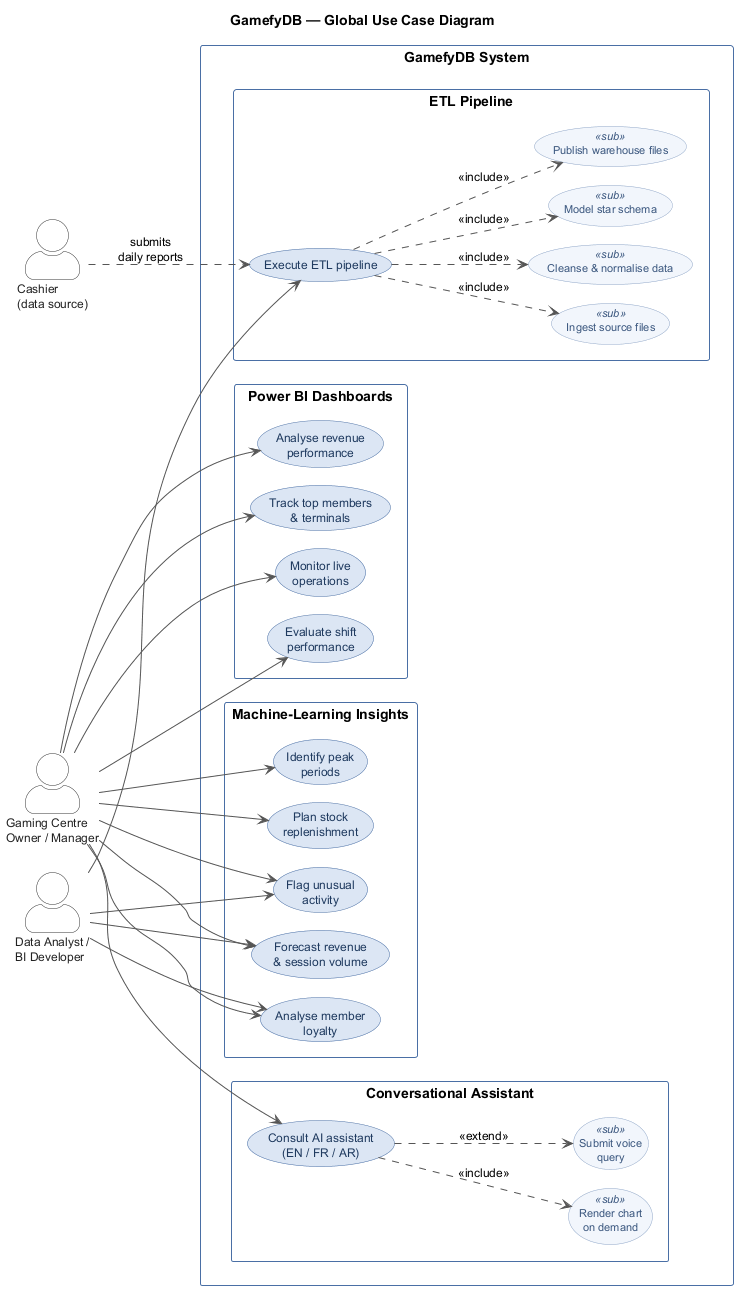
\includegraphics[width=0.95\textwidth]{images/use_cases.png}
  \caption{Global use case diagram for GamefyDB.}
  \label{fig:usecase}
\end{figure}

The three actors are stacked on the left of the system boundary; the
right-hand side groups the use cases into four packages that mirror the
project's four sprints: \textit{ETL Pipeline}, \textit{Power BI Dashboards},
\textit{Machine-Learning Insights}, and \textit{Conversational Assistant}.
The \textit{Cashier} is upstream of everything else: they generate the daily
exports that feed the pipeline, and only interact with the
\textit{Execute ETL pipeline} use case. The \textit{Analyst} triggers the
pipeline and drives the ML use cases (forecasts, segmentation, anomaly
detection). The \textit{Owner / Manager} is the broadest consumer: they
read every dashboard, every ML output, and query the conversational
assistant. Two composition patterns are visible on the right of the
diagram. \textit{Execute ETL pipeline} expands into its four sub-steps
(ingest, cleanse, transform, publish) via \texttt{<<include>>} arrows.
The conversational assistant always renders a chart on demand
(\texttt{<<include>>}) and optionally accepts a voice query
(\texttt{<<extend>>}).

\section{Project Management with Scrum}

\subsection{Identification of the Scrum Team}

\begin{itemize}
  \item \textbf{Product Owner}: \textbf{Mr.\ Aymen Jadallah}, owner of Gamefy
        Academy. He defined the business requirements, reviewed every sprint
        increment, and validated that the dashboards and the chatbot answered
        the kinds of questions he actually asks.

  \item \textbf{Scrum Master}: \textbf{Mr.\ Sofien Boutaib}, PhD in Computer
        Science from ISIMA and my academic supervisor. He made sure the Scrum
        ceremonies were respected and provided methodological and technical
        guidance throughout.

  \item \textbf{Development Team}: \textbf{Sarra Mediouni}, sole developer
        responsible for the pipeline, the ML modules, the Power~BI report,
        and the chatbot.
\end{itemize}

\subsection{Product Backlog}

The product backlog is the ordered list of every user story the project needs
to deliver. Sprint~4 (ML) and Sprint~5 (chatbot) were not in the original
backlog — they were added after Sprint~3 was validated, at the Product
Owner's request, once he could see what was possible on top of the cleaned
data.

\begin{longtable}{>{\bfseries}p{1.3cm} p{4.6cm} p{6.6cm} c}
  \caption{Product Backlog.\label{tab:backlog}} \\
  \toprule
  \textbf{ID} & \textbf{User Story} & \textbf{Tasks} & \textbf{Sprint} \\
  \midrule
  \endfirsthead
  \toprule
  \textbf{ID} & \textbf{User Story} & \textbf{Tasks} & \textbf{Sprint} \\
  \midrule
  \endhead
  \bottomrule
  \endfoot

  US-01 & As an analyst, I want to read all four source files without errors.
        & Implement one loader function per file in \texttt{pipeline.py};
          map column indices empirically.
        & 1 \\[3pt]
  US-02 & As an analyst, I want page-break artefacts removed automatically.
        & Implement \texttt{\_is\_header\_row()} and filter inside each loader.
        & 1 \\[3pt]
  US-03 & As an analyst, I want amounts, dates, and durations correctly typed.
        & Implement \texttt{\_parse\_amount()} and \texttt{\_parse\_duration()}.
        & 1 \\[3pt]
  US-04 & As an analyst, I want missing cashier names corrected.
        & Implement \texttt{\_fill\_cashier()} with forward/backward fill.
        & 1 \\[3pt]
  US-05 & As an analyst, I want four dimension tables with surrogate keys.
        & Build the dims inside \texttt{build\_star\_schema()}.
        & 2 \\[3pt]
  US-06 & As an analyst, I want two fact tables with FK references.
        & Build \textit{fact\_transaction} and \textit{fact\_session};
          resolve all FKs; use nullable \texttt{Int64} for optional refs.
        & 2 \\[3pt]
  US-07 & As an analyst, I want the schema exported as UTF-8-BOM CSV files.
        & Write the six tables to \texttt{output/powerbi\_star/} from
          \texttt{run.py}.
        & 2 \\[3pt]
  US-08 & As an owner, I want KPIs visualised in interactive dashboards.
        & Build \texttt{gamefyyy.pbix}: date dim, relationships, DAX measures,
          four dashboard pages.
        & 3 \\[3pt]
  US-09 & As an owner, I want a revenue forecast for the next 4 weeks and 3 months.
        & Implement \texttt{forecast\_revenue()} with Prophet.
        & 4 \\[3pt]
  US-10 & As an owner, I want to forecast member activity.
        & Implement \texttt{forecast\_members()} on weekly aggregates.
        & 4 \\[3pt]
  US-11 & As an owner, I want to see the busiest hours and days.
        & Implement \texttt{forecast\_peak\_hours()} returning two CSVs.
        & 4 \\[3pt]
  US-12 & As an owner, I want a forecast of total daily activity volume.
        & Implement \texttt{forecast\_session\_volume()} with Prophet.
        & 4 \\[3pt]
  US-13 & As an owner, I want a restocking recommendation per item.
        & Implement \texttt{forecast\_stock\_replenishment()}.
        & 4 \\[3pt]
  US-14 & As a data analyst, I want two more forecasting models for an
          objective comparison.
        & Implement SARIMA via \texttt{auto\_arima} and XGBoost with engineered
          features; evaluate Prophet vs SARIMA vs XGBoost on an 80/20
          chronological split (MAE, RMSE, wMAPE).
        & 4 \\[3pt]
  US-15 & As an owner, I want forecasts that take weather into account.
        & Add an Open-Meteo Tunis weather client (\texttt{weather.py});
          plug max-temperature + precipitation into Prophet and XGBoost as
          regressors.
        & 4 \\[3pt]
  US-16 & As an owner, I want to know which members are my most valuable.
        & Implement K-Means segmentation (k=4) in \texttt{segmenter.py};
          assign human-readable labels; export segments and per-member
          loyalty scores.
        & 4 \\[3pt]
  US-17 & As an owner, I want to be alerted on abnormally high or low days.
        & Implement day-of-week Z-score detection in
          \texttt{anomaly\_detector.py}; classify mild vs severe; export
          flagged dates to CSV.
        & 4 \\[3pt]
  US-18 & As an owner, I want to ask questions in plain language and get
          answers and charts back.
        & Build a Streamlit assistant (\texttt{app.py}); wire it to the
          star schema, the forecasts, the segments, and the anomalies.
        & 5 \\[3pt]
  US-19 & As an owner, I want to use the assistant in EN, FR, or AR.
        & Translate the UI strings and prompt the underlying agent in the
          selected language.
        & 5 \\[3pt]
  US-20 & As an owner, I want to talk to the assistant instead of typing.
        & Add a voice-input component to the Streamlit app
          (\texttt{chatbot/voice\_component.py}).
        & 5 \\[3pt]
  US-21 & As an owner, I want the assistant to draw a chart on demand.
        & Implement \texttt{chatbot/chart\_generator.py} so the agent can
          return a Plotly Express chart alongside a textual answer.
        & 5 \\
\end{longtable}

\subsection{Sprints Planning}

The project ran over five implementation sprints after Sprint~0:

\begin{itemize}
  \item \textbf{Sprint~1 — Data Loading and Cleaning}: the four loader
        functions, the artefact-filtering logic, the type-conversion helpers,
        and the cashier correction.
  \item \textbf{Sprint~2 — Star Schema and Export}: the dimensional model
        builder and the CSV export step, with referential-integrity checks
        across the six tables.
  \item \textbf{Sprint~3 — Power~BI Dashboards}: the full interactive report,
        the DAX measures, and KPI validation with the Product Owner.
  \item \textbf{Sprint~4 — Machine Learning and Analytics}: the five
        forecasting functions, the SARIMA / XGBoost comparison, the weather
        regressor, the K-Means segmentation, the loyalty score, and the
        Z-score anomaly detector.
  \item \textbf{Sprint~5 — Conversational Assistant}: the Streamlit chatbot
        with multilingual support (EN/FR/AR), voice input, and on-demand
        chart generation.
\end{itemize}

\subsection{Project Planning}

Table~\ref{tab:planning} shows the sprint schedule.

\begin{table}[H]
  \centering
  \caption{Sprint schedule.\label{tab:planning}}
  \begin{tabular}{lll}
    \toprule
    \textbf{Phase}  & \textbf{Start} & \textbf{End} \\
    \midrule
    Sprint 0 — Preparation                  & 02/02/2026 & 14/02/2026 \\
    Sprint 1 — Loading \& Cleaning          & 15/02/2026 & 02/03/2026 \\
    Sprint 2 — Star Schema \& Export        & 03/03/2026 & 12/03/2026 \\
    Sprint 3 — Power~BI Dashboards          & 13/03/2026 & 16/04/2026 \\
    Sprint 4 — ML and Analytics             & 17/04/2026 & 06/05/2026 \\
    Sprint 5 — Conversational Assistant     & 07/05/2026 & 17/05/2026 \\
    \bottomrule
  \end{tabular}
\end{table}

% *TODO* insert Gantt chart image here
% \begin{figure}[H]
%   \centering
%   
\includegraphics[width=\textwidth]{images/gantt.png}
%   \caption{Project Gantt chart.}
%   \label{fig:gantt}
% \end{figure}

\section{Technical Architecture}

Figure~\ref{fig:architecture} shows the overall architecture of the GamefyDB
solution.

\begin{figure}[H]
  \centering
  
\includegraphics[width=0.95\textwidth]{images/pipeline.png}
  \caption{Technical architecture of the GamefyDB solution.}
  \label{fig:architecture}
\end{figure}

The design is intentionally flat. The source layer is just the four Excel
files in \texttt{excel/} (plus a \texttt{weather\_tunis.parquet} cache and a
set of synthetic \texttt{extended\_*.xlsx} files used to give the time-series
models enough history). The processing layer is a handful of focused Python
modules — \texttt{pipeline.py} for the ETL, \texttt{forecaster.py} /
\texttt{segmenter.py} / \texttt{anomaly\_detector.py} for the ML layer,
\texttt{weather.py} for the regressor — all driven by \texttt{run.py}. The
output layer is two folders (\texttt{output/powerbi\_star/} for the star
schema and \texttt{output/forecasts/} for the ML outputs) that Power~BI and
the chatbot both read from directly.

Keeping the ETL in a single module rather than splitting it across four
ingest/clean/transform/export files was a deliberate choice. The cleaning
logic for each source file is tightly coupled to how that file is structured;
forcing it into a generic cleaner would have added abstraction without adding
clarity, and the column-index mappings are easier to maintain side by side
in one place.

\section{Overall Design of the Data Warehouse}

\subsection{Data Collection}

The source data is four \texttt{.xls} files exported by the centre's
point-of-sale software, covering activity from June~2025 through April~2026.
Table~\ref{tab:sourcefiles} summarises them.

\begin{table}[H]
  \centering
  \caption{Source files and their contents.\label{tab:sourcefiles}}
  \begin{tabular}{p{3.5cm} p{9cm}}
    \toprule
    \textbf{File} & \textbf{Contents} \\
    \midrule
    \texttt{14-06-2025 cash.xls}
      & One row per cash transaction. Columns include cashier, datetime,
        income/expense type, payment method, category, and TND amount. \\[4pt]
    \texttt{14-06-2025 session.xls}
      & One row per gaming session. Columns include cashier, terminal,
        session type, duration, and revenue broken down into usage, orders,
        USB data, and discount. \\[4pt]
    \texttt{14-06-2025 stock.xls}
      & One row per stock movement. Columns include cashier, datetime, item
        name, category, direction (in/out), quantity, unit price, and total. \\[4pt]
    \texttt{memeber DATA 01-09-2025.xls}
      & One row per loyalty member. Cumulative stats: total session duration,
        usage spend, order spend, USB spend, total spend. (The typo
        \textit{memeber} is in the real filename and is kept as-is.) \\
    \bottomrule
  \end{tabular}
\end{table}

\subsection{Key Performance Indicators (KPIs)}

The KPIs were defined during Sprint~0 in discussion with the Product Owner.
They fall into four groups for the descriptive side and one for the
forward-looking side. Table~\ref{tab:kpis} summarises them.

\begin{table}[H]
  \centering
  \caption{KPI groups and their measures.\label{tab:kpis}}
  \begin{tabular}{p{3cm} p{10cm}}
    \toprule
    \textbf{Group} & \textbf{KPIs} \\
    \midrule
    Revenue
      & Total income (TND), total expenses (TND), net income, revenue by
        payment method, revenue by cashier, revenue by transaction category,
        month-over-month revenue change, average transaction value. \\[4pt]
    Sessions
      & Total session count, average session duration (minutes), free-vs-paid
        split, total discount given, session revenue by terminal and by
        terminal type. \\[4pt]
    Stock
      & Total units sold per item, total snack-bar revenue, average unit
        price per item, current stock level. \\[4pt]
    Members
      & Active members, average spend per member, total session duration
        across all members, orders transferred, USB-data usage, loyalty score
        distribution. \\[4pt]
    Forward-looking
      & Revenue forecast (4~weeks / 3~months) with confidence interval,
        member-activity forecast, peak-hour and peak-day profile, per-item
        restocking recommendation, anomaly-flagged dates by series and
        severity. \\
    \bottomrule
  \end{tabular}
\end{table}

\subsection{Data Warehouse Design Approaches}

\subsubsection{Inmon Approach}

Bill Inmon's approach, often called \textit{top-down}, starts by designing a
single fully normalised enterprise data warehouse covering the whole
organisation, then derives subject-oriented data marts from it. Normalisation
keeps the redundancy low and gives a single source of truth, but it requires
the entire warehouse to be designed before any reports can be produced.

\subsubsection{Kimball Approach}

Ralph Kimball's approach, \textit{bottom-up}, models each business process as
an independent star schema and integrates them later through shared conformed
dimensions. It gets usable output into analysts' hands much faster, at the
cost of some potential redundancy between data marts.

\subsubsection{Adopted Approach}

I went with \textbf{Kimball}. With only four business domains, one physical
location, and a tight project timeline, designing a full normalised EDW
first would have taken the entire internship without producing any
dashboards. The bottom-up approach let me validate each output table against
the real data during Sprint~2 and adjust before moving on. The shared
\textit{dim\_cashier} and \textit{dim\_terminal} dimensions provide the
cross-domain integration that Kimball requires, without adding the complexity
of a fully normalised warehouse on top.

\section{Multidimensional Modelling}

\subsection{Conceptual Model Analysis}

Three dimensional schema patterns were evaluated:

\begin{itemize}
  \item \textbf{Star schema} — fact tables reference dimension tables directly,
        no further normalisation. Simple, fast, easy to understand. This is
        what Power~BI is optimised for.

  \item \textbf{Snowflake schema} — dimensions are further normalised into
        sub-dimensions. Saves some storage but adds joins at query time.
        Power~BI handles joins, but each extra one adds a little complexity
        to the model.

  \item \textbf{Galaxy (fact-constellation) schema} — multiple fact tables
        share conformed dimensions. This is essentially what GamefyDB needs,
        because both fact tables share the cashier, terminal, and member
        dimensions.
\end{itemize}

\subsection{Choice of Conceptual Model}

The model adopted is a \textbf{galaxy / fact-constellation schema}: two fact
tables (\textit{fact\_transaction} and \textit{fact\_session}) share three
conformed dimensions (\textit{dim\_cashier}, \textit{dim\_terminal},
\textit{dim\_member}), while \textit{dim\_item} is referenced from
\textit{fact\_transaction} only (for order-income rows). Stock movements and
per-member cumulative statistics were absorbed directly into the
\textit{dim\_item} and \textit{dim\_member} dimensions during the design
refinement of Sprint~2 — there is only one direction of stock movement
(out-of-stock sales) and the members file is cumulative rather than
event-based, so dedicated fact tables for them would have added complexity
without analytical value.

Figure~\ref{fig:starschema} shows the full conceptual model.

\begin{figure}[H]
  \centering
  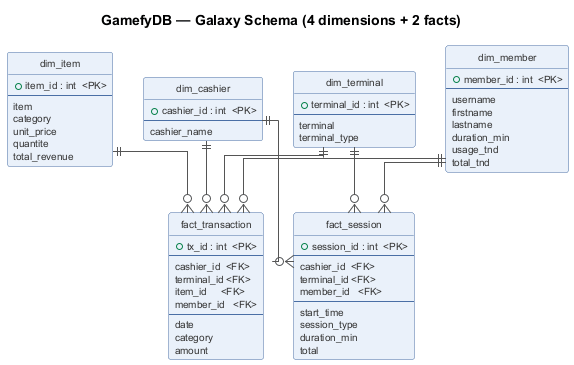
\includegraphics[width=\textwidth]{images/star_schema.png}
  \caption{Conceptual model of the GamefyDB data warehouse.}
  \label{fig:starschema}
\end{figure}

Table~\ref{tab:star_schema} lists the six output tables and their key columns.

\begin{table}[H]
  \centering
  \caption{Output tables of the GamefyDB star schema.\label{tab:star_schema}}
  \begin{tabular}{lll}
    \toprule
    \textbf{Type} & \textbf{Table} & \textbf{Key columns} \\
    \midrule
    Dimension & \texttt{dim\_cashier}  & cashier\_id (PK), cashier\_name \\
    Dimension & \texttt{dim\_terminal} & terminal\_id (PK), terminal, terminal\_type \\
    Dimension & \texttt{dim\_item}     & item\_id (PK), item, category, unit\_price, \\
              &                        & quantite, total\_revenue \\
    Dimension & \texttt{dim\_member}   & member\_id (PK), username, firstname, lastname, \\
              &                        & duration\_min, usage\_tnd, orders\_tnd, total\_tnd \\
    \midrule
    Fact & \texttt{fact\_transaction} & tx\_id (PK), cashier\_id (FK),
                                        terminal\_id (FK, nullable), \\
         &                            & item\_id (FK, nullable),
                                        member\_id (FK, nullable), \\
         &                            & date, category, amount \\
    Fact & \texttt{fact\_session}     & session\_id (PK), cashier\_id (FK),
                                        terminal\_id (FK), \\
         &                            & member\_id (FK, nullable),
                                        session\_type, duration\_min, \\
         &                            & order\_transfer, usage, discount, total \\
    \bottomrule
  \end{tabular}
\end{table}

\section{Work Environment}

\subsection{Hardware Environment}

\begin{itemize}[noitemsep]
  \item Machine: Lenovo laptop, model 83DV
  \item Processor: Intel Core i7-13650HX (13th gen), 14 cores / 20 threads
  \item RAM: 32~GB
  \item Storage: 500~GB MSI M450 SSD + 512~GB Micron NVMe SSD
  \item GPU: NVIDIA GeForce RTX 4050 Laptop
  \item Operating system: Windows~11 Pro
\end{itemize}

\subsection{Software Environment}

\begin{itemize}
  \item \textbf{Python 3.x} — main implementation language for the pipeline,
        the ML modules, the chatbot, and the helper scripts.
  \item \textbf{pandas} and \textbf{NumPy} — used throughout for reading the
        source files, all DataFrame operations, vectorised nearest-neighbour
        FK matching, and CSV/Excel output.
  \item \textbf{openpyxl} — reads and writes the \texttt{.xlsx} extended files
        produced by the synthetic data generator.
  \item \textbf{Prophet} (Meta) — additive time-series model used to forecast
        revenue, member activity, and session volume, with the Open-Meteo
        weather regressor.
  \item \textbf{pmdarima} — wraps an \texttt{auto\_arima} SARIMA fitting
        routine used as the comparison baseline for Prophet.
  \item \textbf{XGBoost} — gradient-boosting model used as a third
        comparison algorithm, with engineered lag and weather features.
  \item \textbf{statsmodels} — provides the Augmented Dickey-Fuller test
        used for the stationarity study in Sprint~4.
  \item \textbf{scikit-learn} — provides K-Means and the preprocessing
        utilities used by the member segmentation.
  \item \textbf{matplotlib} — generates all the accuracy, segmentation,
        peak-hour, and anomaly-timeline figures shipped with the report.
  \item \textbf{requests} — calls the Open-Meteo API for daily Tunis weather
        and caches the result in a parquet file.
  \item \textbf{Streamlit} — runs the conversational assistant
        (\texttt{app.py}), including the multilingual UI and the voice-input
        component.
  \item \textbf{Power~BI Desktop} — loads the star schema and the analytics
        CSVs, defines the relationships, writes the DAX measures, and assembles
        the four-page interactive report (\texttt{gamefyyy.pbix}).
  \item \textbf{pytest} — automated testing for the parsing, cleaning,
        segmentation, anomaly, and weather modules.
  \item \textbf{VS~Code} — code editor with the Python and PlantUML extensions.
  \item \textbf{PlantUML} — diagramming tool used to generate the use-case,
        pipeline-architecture, and star-schema diagrams from
        \texttt{.puml} sources.
  \item \textbf{Git / GitHub} — version control and remote repository hosting
        for all code and documentation.
  \item \textbf{Overleaf} — online \LaTeX{} editor used to write and compile
        this report.
\end{itemize}

\section{Conclusion}

By the end of Sprint~0, the scope was defined, the backlog was in place,
and the architectural decisions had been made. The choice of Kimball over
Inmon, galaxy schema over snowflake, and one unified pipeline module over
separate stage files all came from the same place: the project is small,
the data quality is uncertain, the timeline is short, and adding abstraction
upfront would have slowed everything down without paying for itself.
Chapter~3 covers the first implementation sprint, where the loading and
cleaning work actually started.

% ============================================================
\end{document}
